\section{Kinematics and Timing of Signal and Background events}
\label{sec:kinematics_and_timing}

%% Taritree (9/20/16): The SM abbreaviation is used fo the first time here without introduction.
%% I've added the abbreviation to the introduction.

\subsection{Kinematics of the 0\nbb-decay signal}

We simulate the kinematics of 0\nbb~ events using a custom Monte
Carlo with momentum and angle-dependent phase space
factors for 0\nbb~decay~\cite{Jenni}.  The spectrum in kinetic energy
of the electrons in 0\nbb~ decays of \Te~ is shown in
Figure~\ref{fig:Energy_spectrum}.

\begin{figure*}[ht]
  \centering
  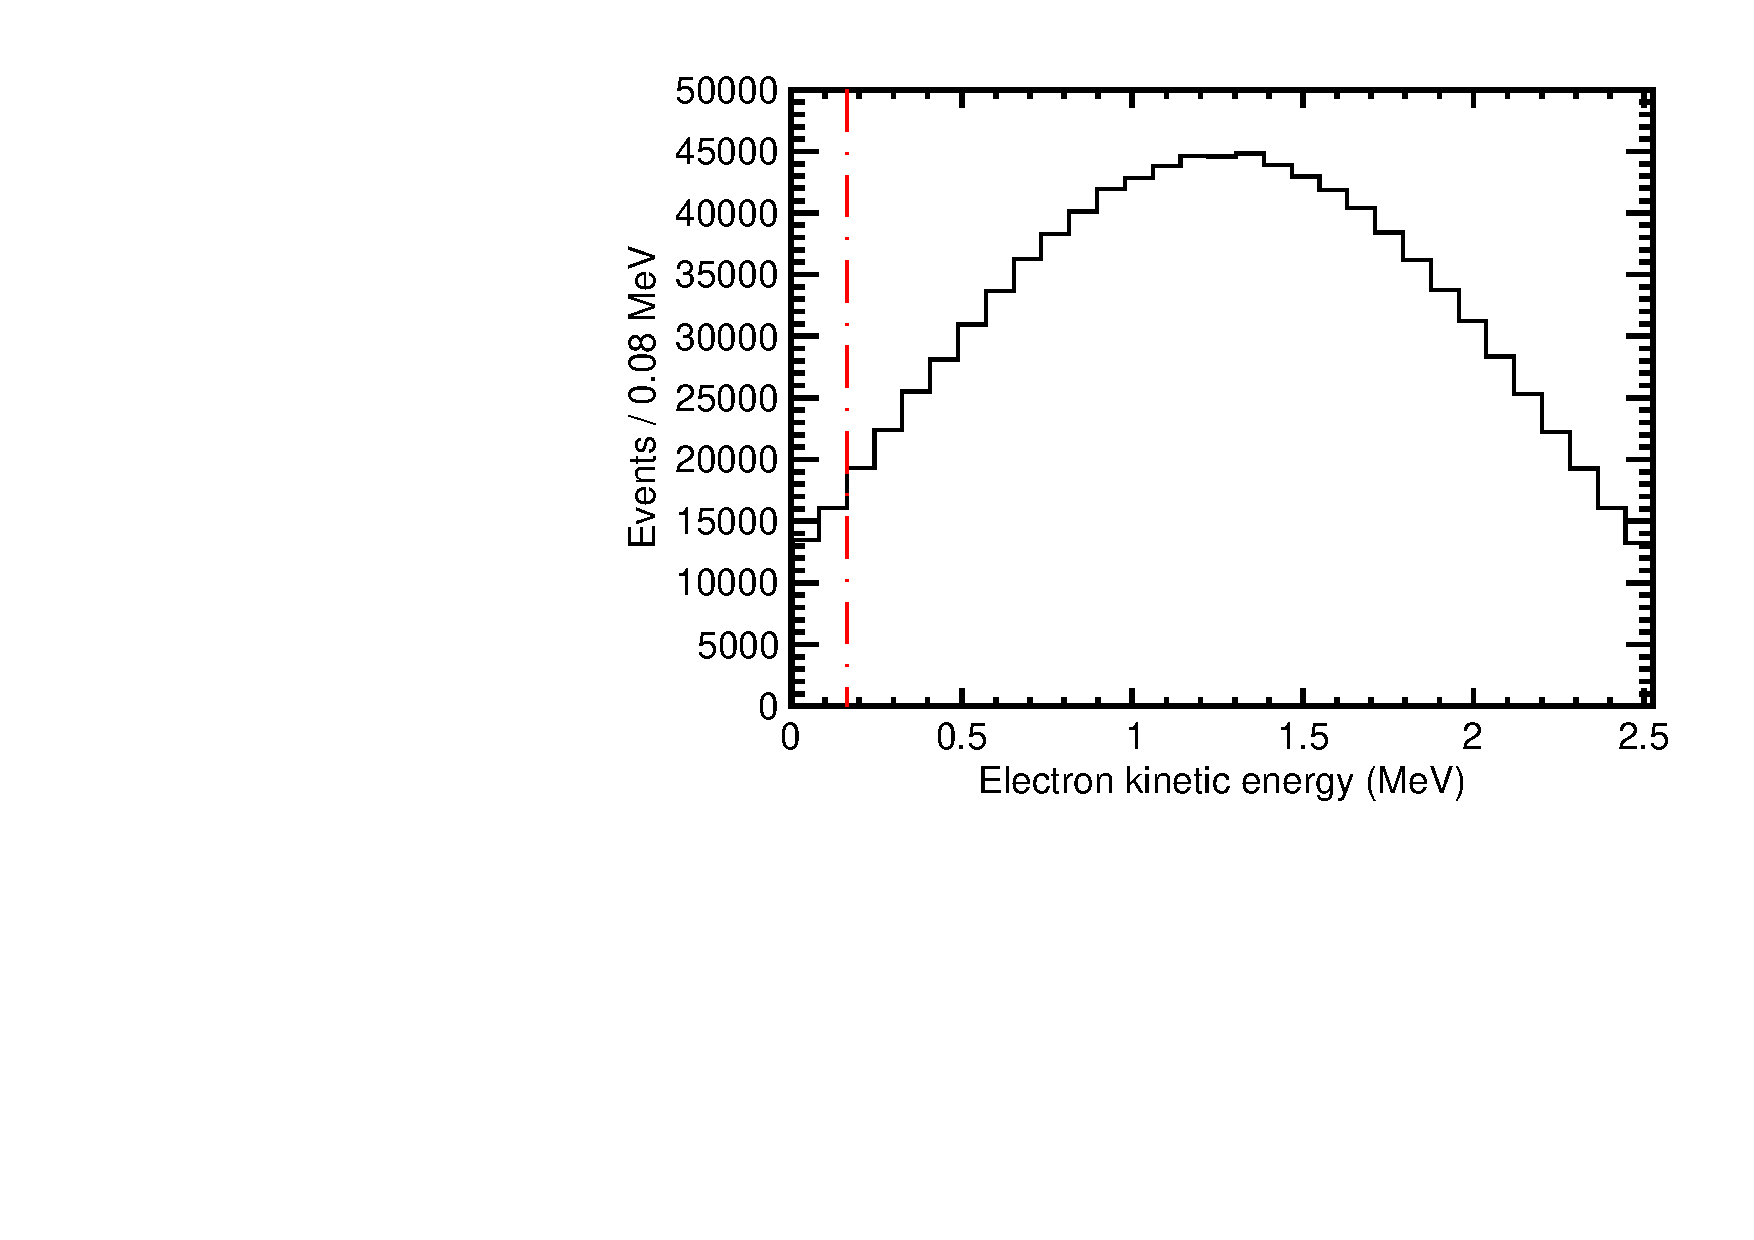
\includegraphics[width=0.65\textwidth]{hK_che_threshold.pdf}
  \caption{The spectrum in kinetic energy of the electrons in 0\nbb~
  decays of \Te~ (endpoint 2.53 MeV). The vertical dashed line
  indicates the Cherenkov threshold in the liquid scintillator of the
  detector model. Single electrons from \B~ solar neutrinos that are
  potential background to the 0\nbb~ search are close in energy to the
  endpoint and will be above the Cherenkov threshold.}
 \label{fig:Energy_spectrum}
\end{figure*}


The distribution in
$\cos{(\theta)}$ between the two electrons is presented in the left-hand
panel of Fig.~\ref{fig:Kinematics} (solid line), showing the
preference towards a back-to-back topology.  The energy sharing between
the electrons peaks at an equal split, as shown in the right-hand
panel of Fig.~\ref{fig:Kinematics} (solid line).

\begin{figure*}[ht]
  \centering
  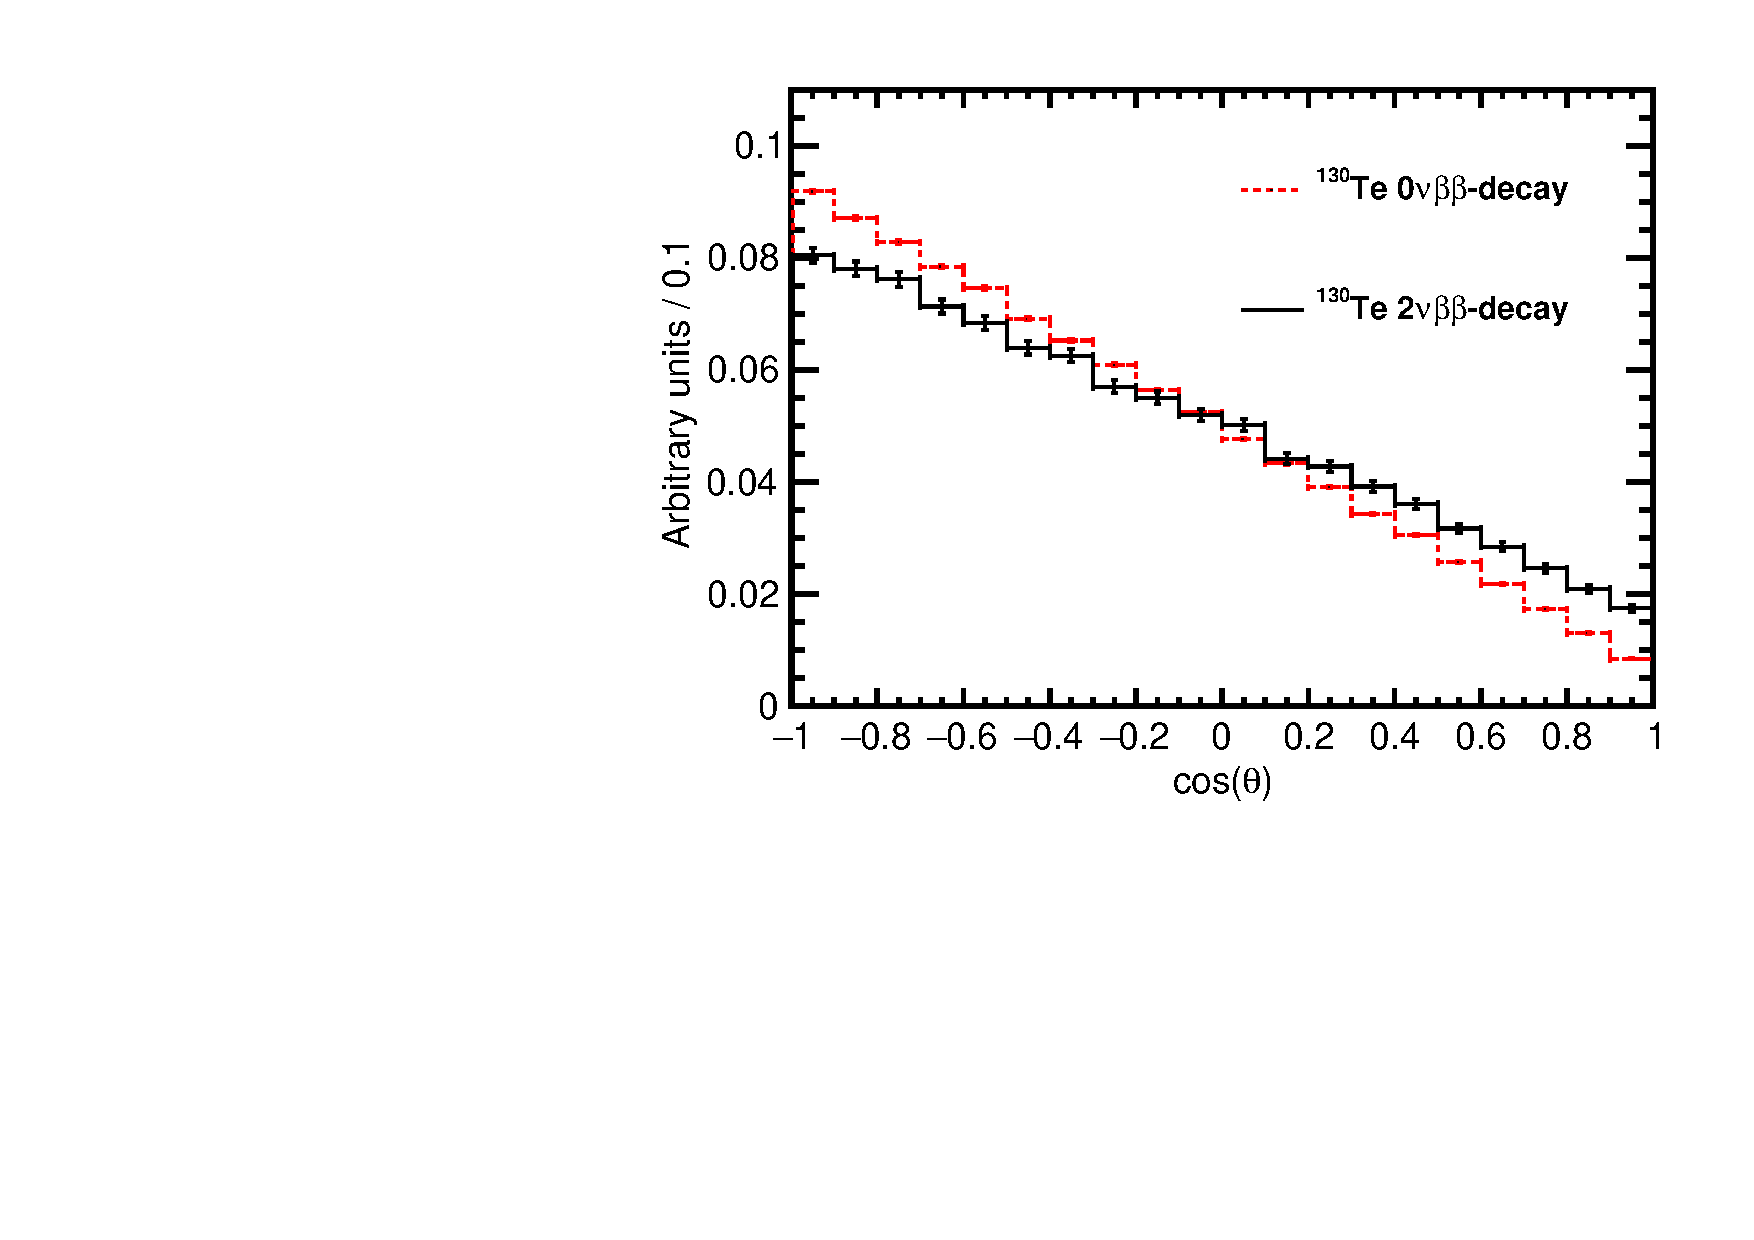
\includegraphics[width=0.49\textwidth]{hCos_Te130.pdf}
  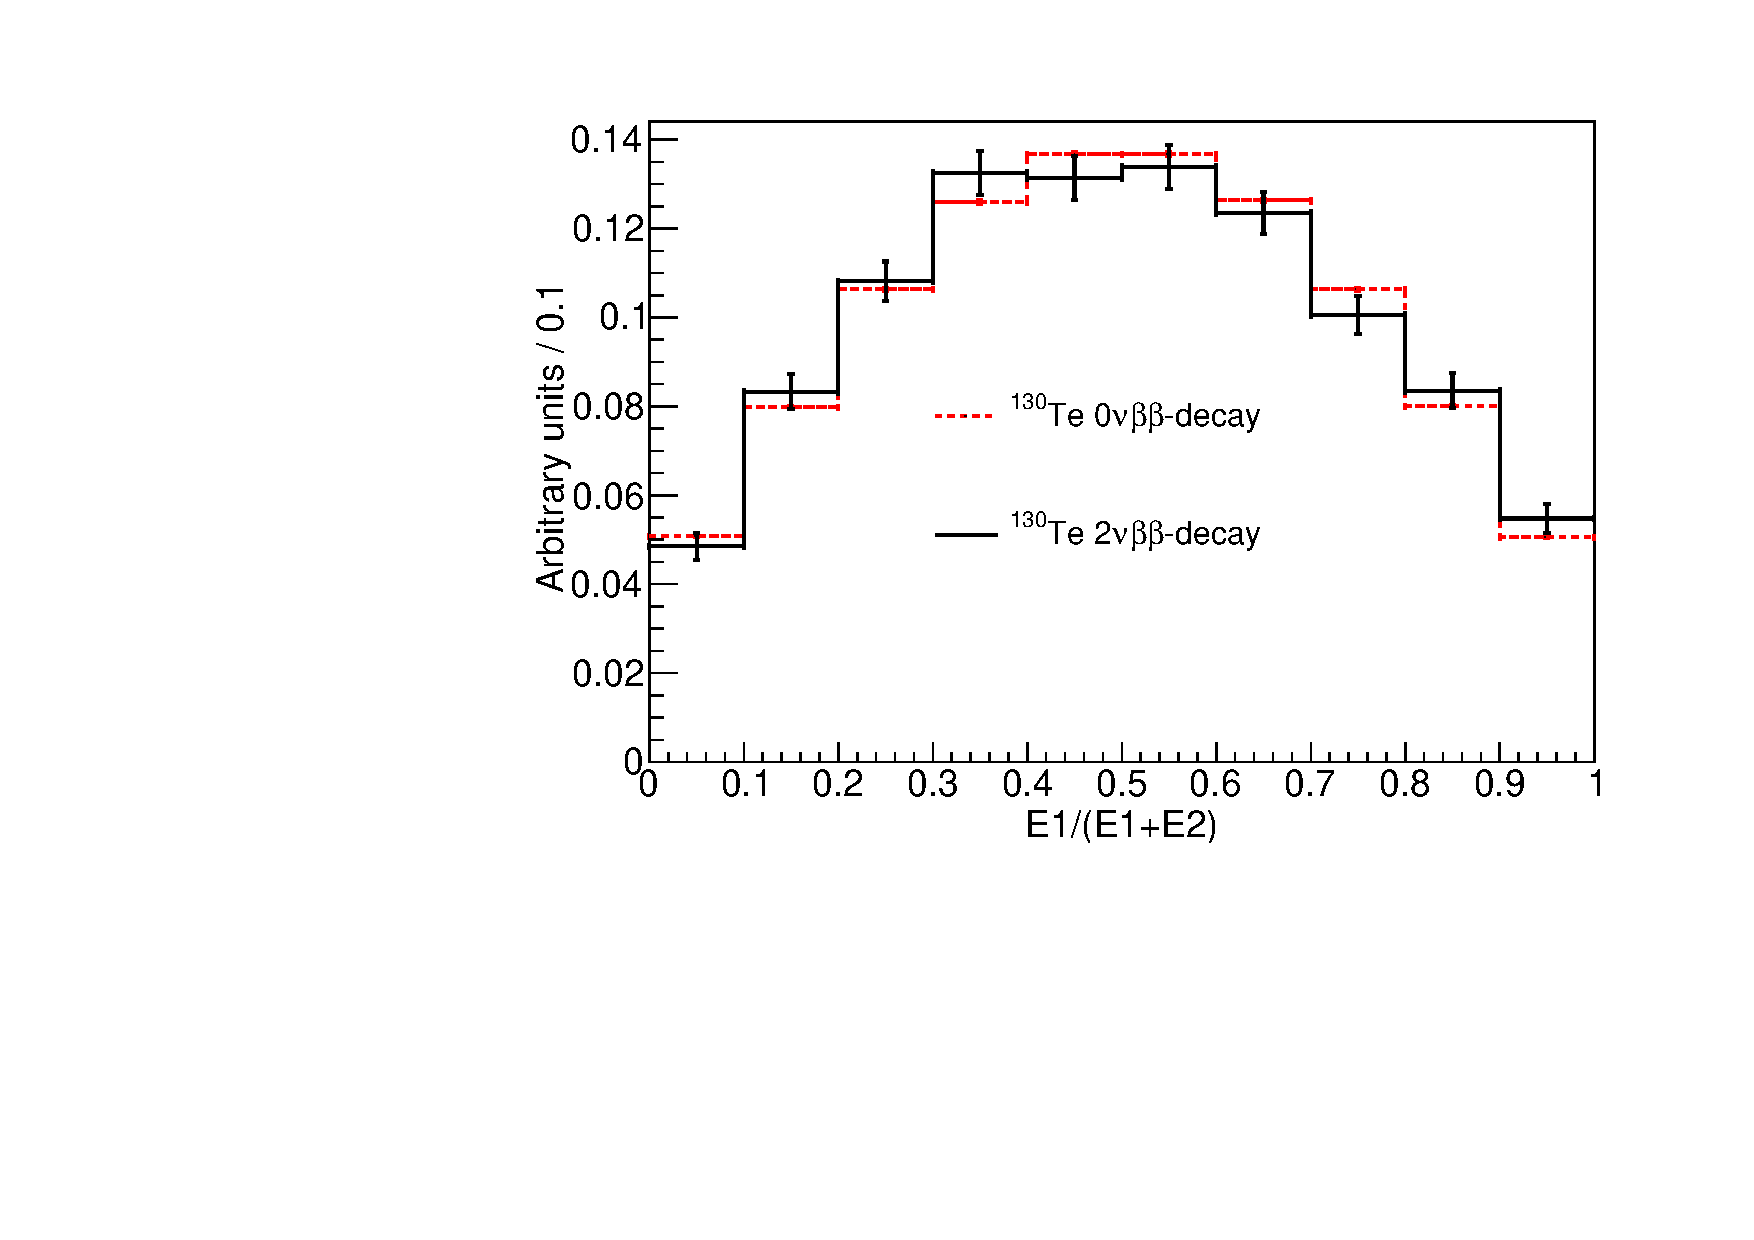
\includegraphics[width=0.49\textwidth]{hE1toQ_Te130.pdf}
  \caption{\emph{Left:} The distribution in the cosine of the angle
      between the two electrons for 0{\nbb} decays (solid black line).
      \emph{Right:} The fraction of the total energy carried by one of
      the two electrons in 0{\nbb} decays (solid black line).  In both
      panels the dashed red line is the corresponding distribution for
      SM 2\nbb~ events with the total kinetic energy of the electrons
      above 90\% of the Q-value.}
  \label{fig:Kinematics}
\end{figure*}

\subsection{Comparison to SM 2\nbb~ decay}
\label{comparison}

Figure~\ref{fig:Kinematics} also shows the angular separation and
energy sharing of the two electrons in SM 1\nbb~ events with the total kinetic
energy of the electrons above 90\% of the Q-value, found using the
same Monte Carlo generator but with SM phase space
factors~\cite{Jenni}.  As seen from the plot, the electron angular
correlations for 0\nbb-decay are slightly more back-to-back than those
from 2\nbb-decay due to a contribution from the neutrino
wave-functions even at vanishingly small energies of the
neutrinos~\cite{Jenni}. The energy sharing is essentially
identical.

\subsection{Production and Selection 
of Cherenkov light by electrons from \Te~ 0\nbb~ decays}
Figure~\ref{fig:Energy_spectrum} also shows the threshold for the
production of Cherenkov light.
Examining the kinematics for one of the electrons from \Te~
0\nbb~decay with an equal energy split, the 1.26~MeV electron travels
on average a total path length of 7.1$\pm$0.9~mm, has a distance from
the origin of 5.6$\pm$1.0~mm in 26 $\pm$4~ps, and takes
24$\pm$3~ps to drop below Cherenkov threshold.  We note that due
to scattering of the electron, the final direction of the electron
before it stops does not correspond to the initial direction; however,
the scattering angle is small at the time that the majority of
Cherenkov light is produced.

Figure~\ref{fig:ArrivalTimeDist} shows distributions from the detector
simulation for 1000 \Te~ 0\nbb-decay events at the center of the
detector. The left-hand panel compares the time of photoelectron (PE)
arrival at a photodetector anode for Cherenkov and scintillation
light, assuming a transit-time spread (TTS)~\cite{TTS} in the
photodetector of 100 ps.  A selection of the PEs with relatively small
arrival time creates a sample with a high fraction of directional
Cherenkov light, designated as the `early PE' sample.

The right-hand panel shows the composition of the early PE sample,
selected with a time cut of 33.5~ns (vertical line on plot). On
average each \Te~ 0\nbb-decay produces 62.8$\pm$0.3 PEs in the early
PE sample, with an RMS width of 8.9 PEs from event-by-event
fluctuations.  On average the early PE sample consists of 28.6$\pm$0.2
scintillation PEs and 34.2$\pm$0.2 Cherenkov PEs, with RMS
distribution widths of 5.2 and 7.3 PEs respectively.


\begin{figure*}[ht]
  \centering
  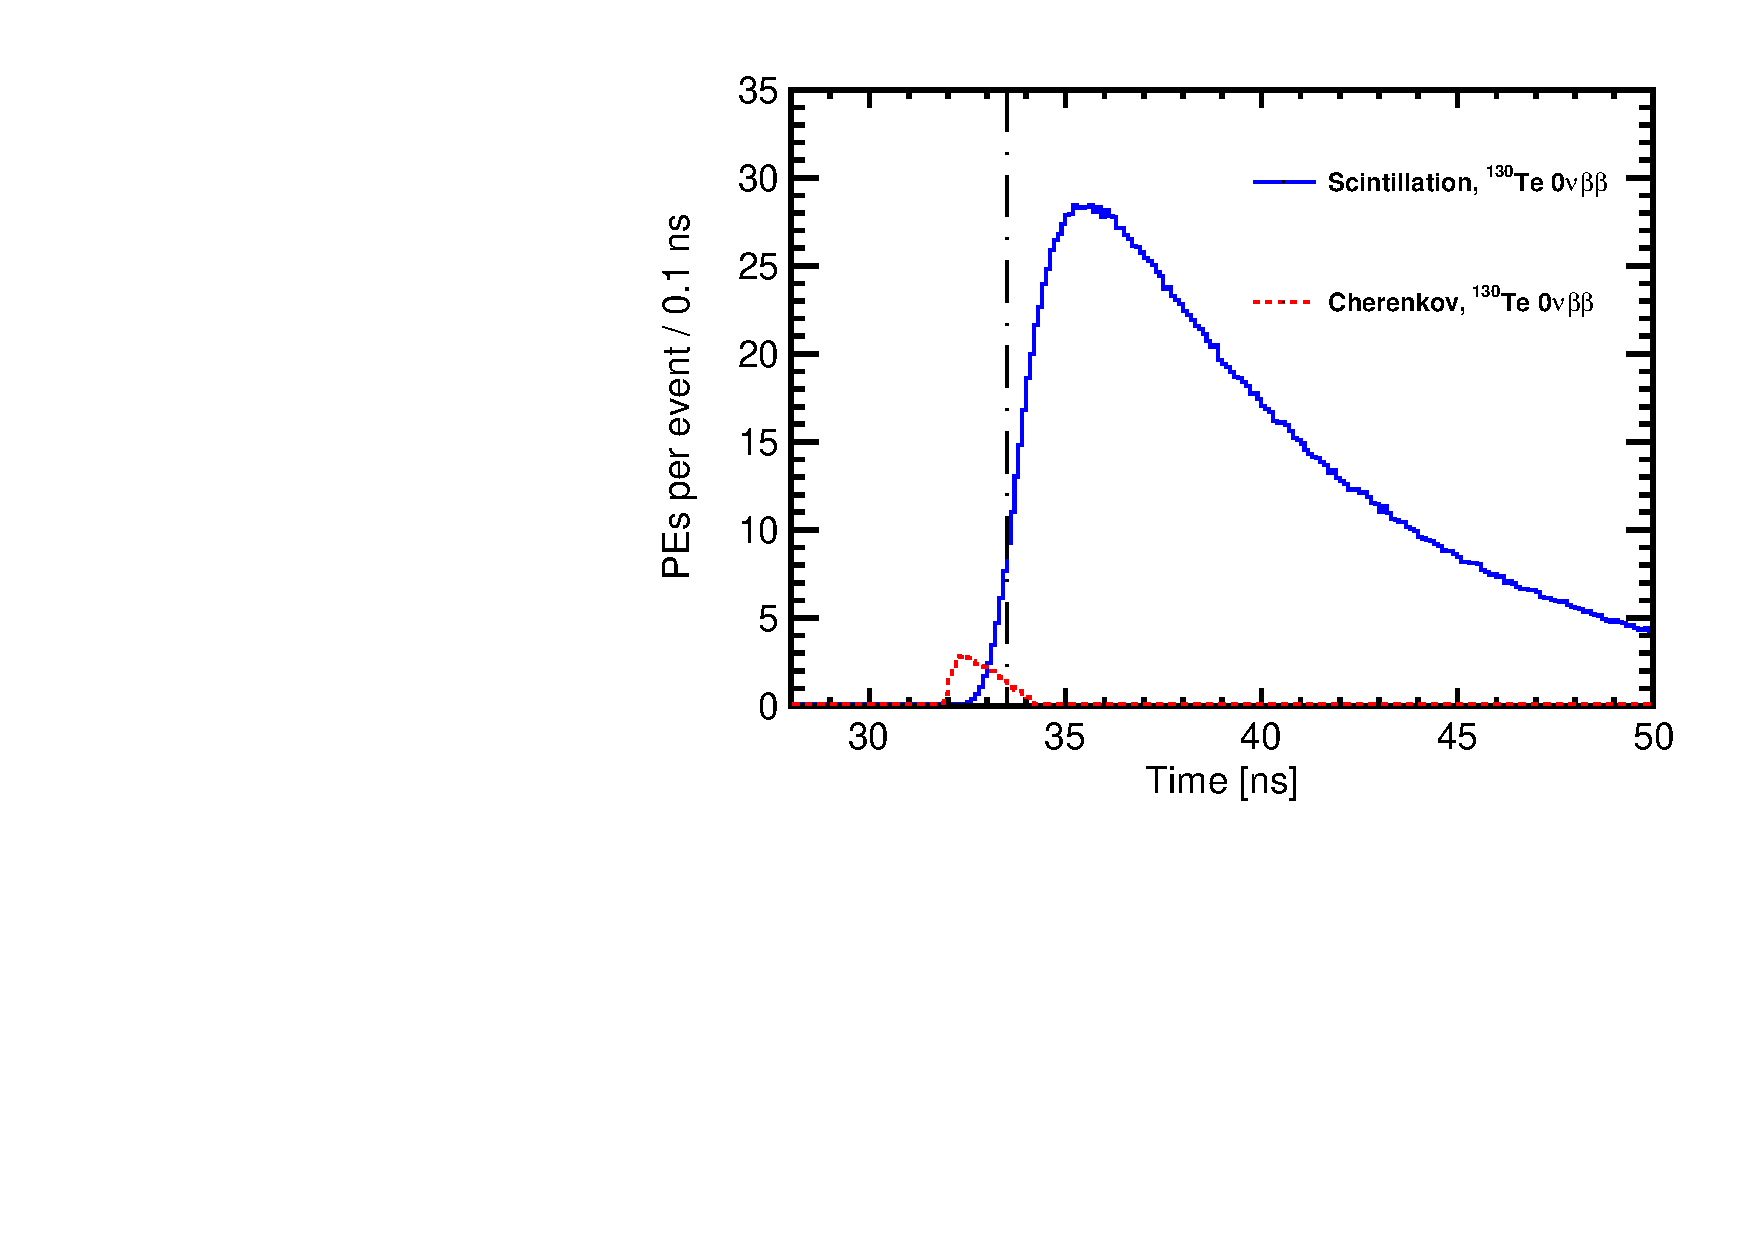
\includegraphics[width=0.45\textwidth]{hT_Te130_v2.pdf}
\hfil
  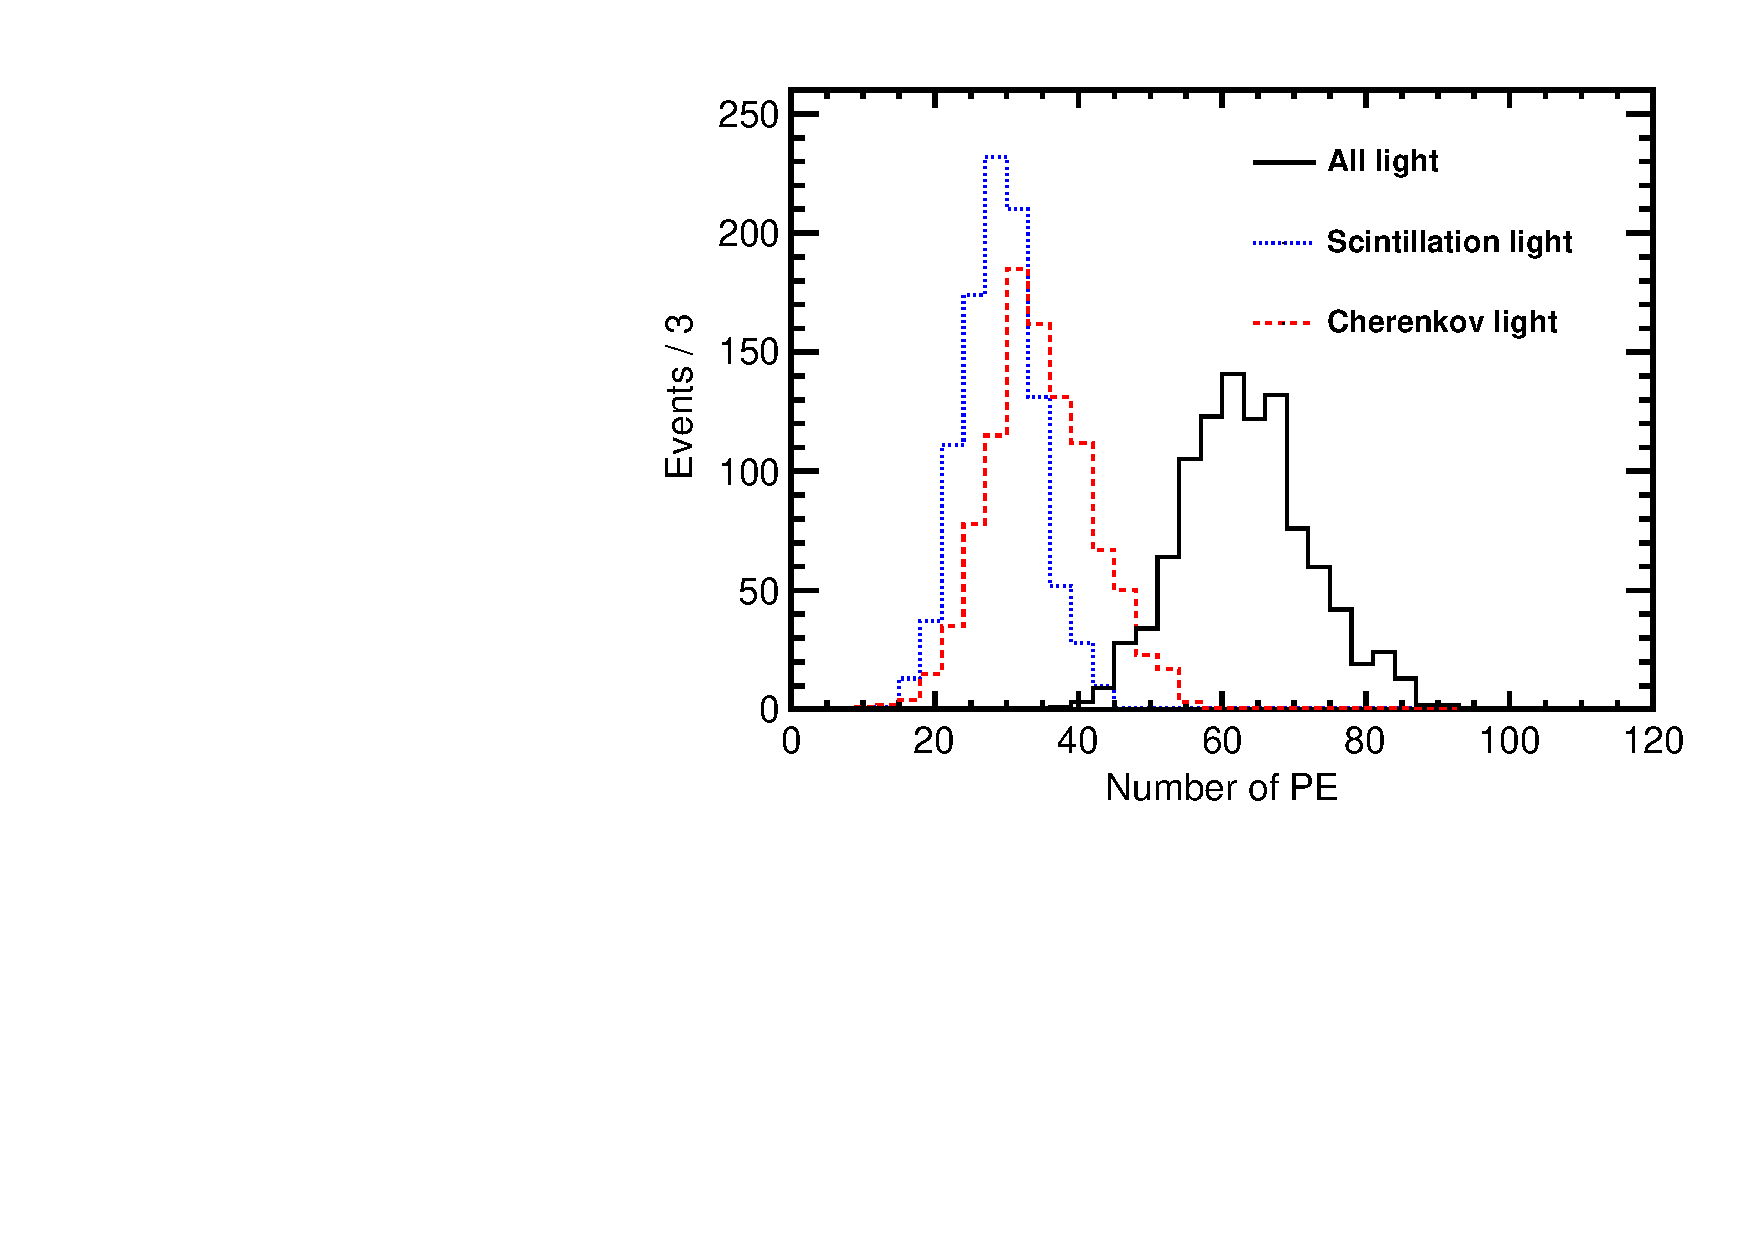
\includegraphics[width=0.45\textwidth]{hMomNPhot_Te130.pdf}
  \caption{\emph{Left:} Photoelectron (PE) arrival times after
    application of the photo-detector transit time spread (TTS) of
    100~ps for the default simulation of \Te~0\nbb-decay produced at
    the center of the detector.  Scintillation PEs (blue solid line)
    are compared to Cherenkov PEs (red dotted line). The vertical line
    at 33.5~ns indicates the time cut for the selection of the early
    PE sample.  \emph{Right:} Composition of the early PE sample (to
    the left of the vertical line in the left-hand panel):
    the number of Cherenkov (\emph{dashed red line}), scintillation
    (\emph{dotted blue line}), and total (\emph{solid black line}) PEs
    per event.}
\label{fig:ArrivalTimeDist}
\end{figure*}


\subsection{\B~ solar neutrino background}

For a detector similar to our model, the \B~solar neutrino background is
significant due to the large total mass of the liquid scintillator in the
active region.  Electrons from elastic scattering of \B~solar
neutrinos have nearly a flat energy spectrum around the
Q-value~\cite{SNOp-B8-bkg}. We simulate \B~background as a single
monochromatic electron with energy of 2.53~MeV (Q-value of \Te). A
2.53~MeV electron travels a total path length of 15.5$\pm$2.0~mm, has
a distance from the origin of 12.6$\pm$2.2~mm in 55$\pm$7~ps, and
takes 49$\pm$2~ps to drop below Cherenkov threshold.

The shape of scintillation and Cherenkov PE timing distributions in
\B~events match very closely the shape of corresponding distributions
for 0\nbb-decay events shown in Fig.~\ref{fig:ArrivalTimeDist}. The
electron path length is too short compared to the detector size to
introduce any noticeable difference in the shape of PE timing
distributions between a single electron from \B~events and two
electrons from 0\nbb-events. 

\begin{figure*}[ht]

  \centering
%  \includegraphics[width=0.45\textwidth]{Che_light_Te130_B8.png}
  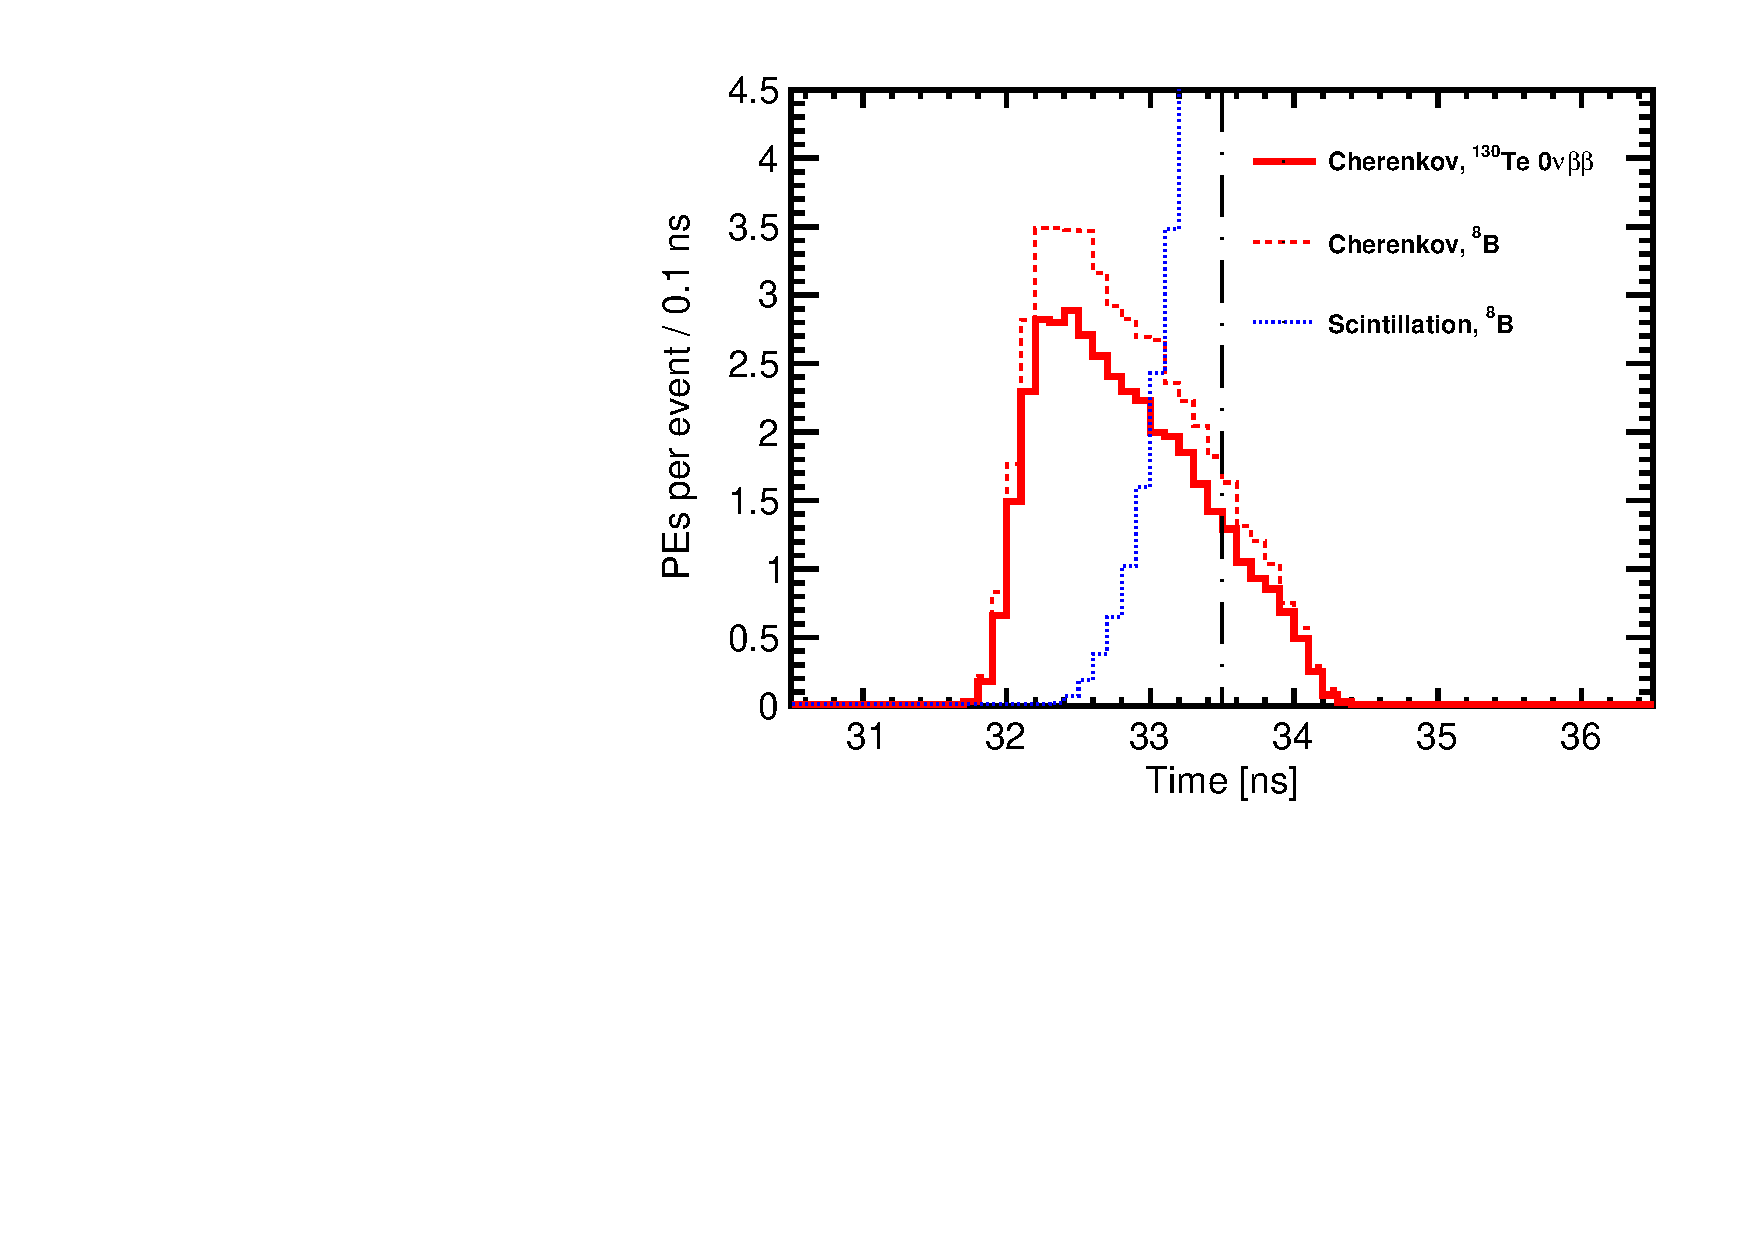
\includegraphics[width=0.45\textwidth]{hTche_Te130_B8_v2.pdf}
\hfil
  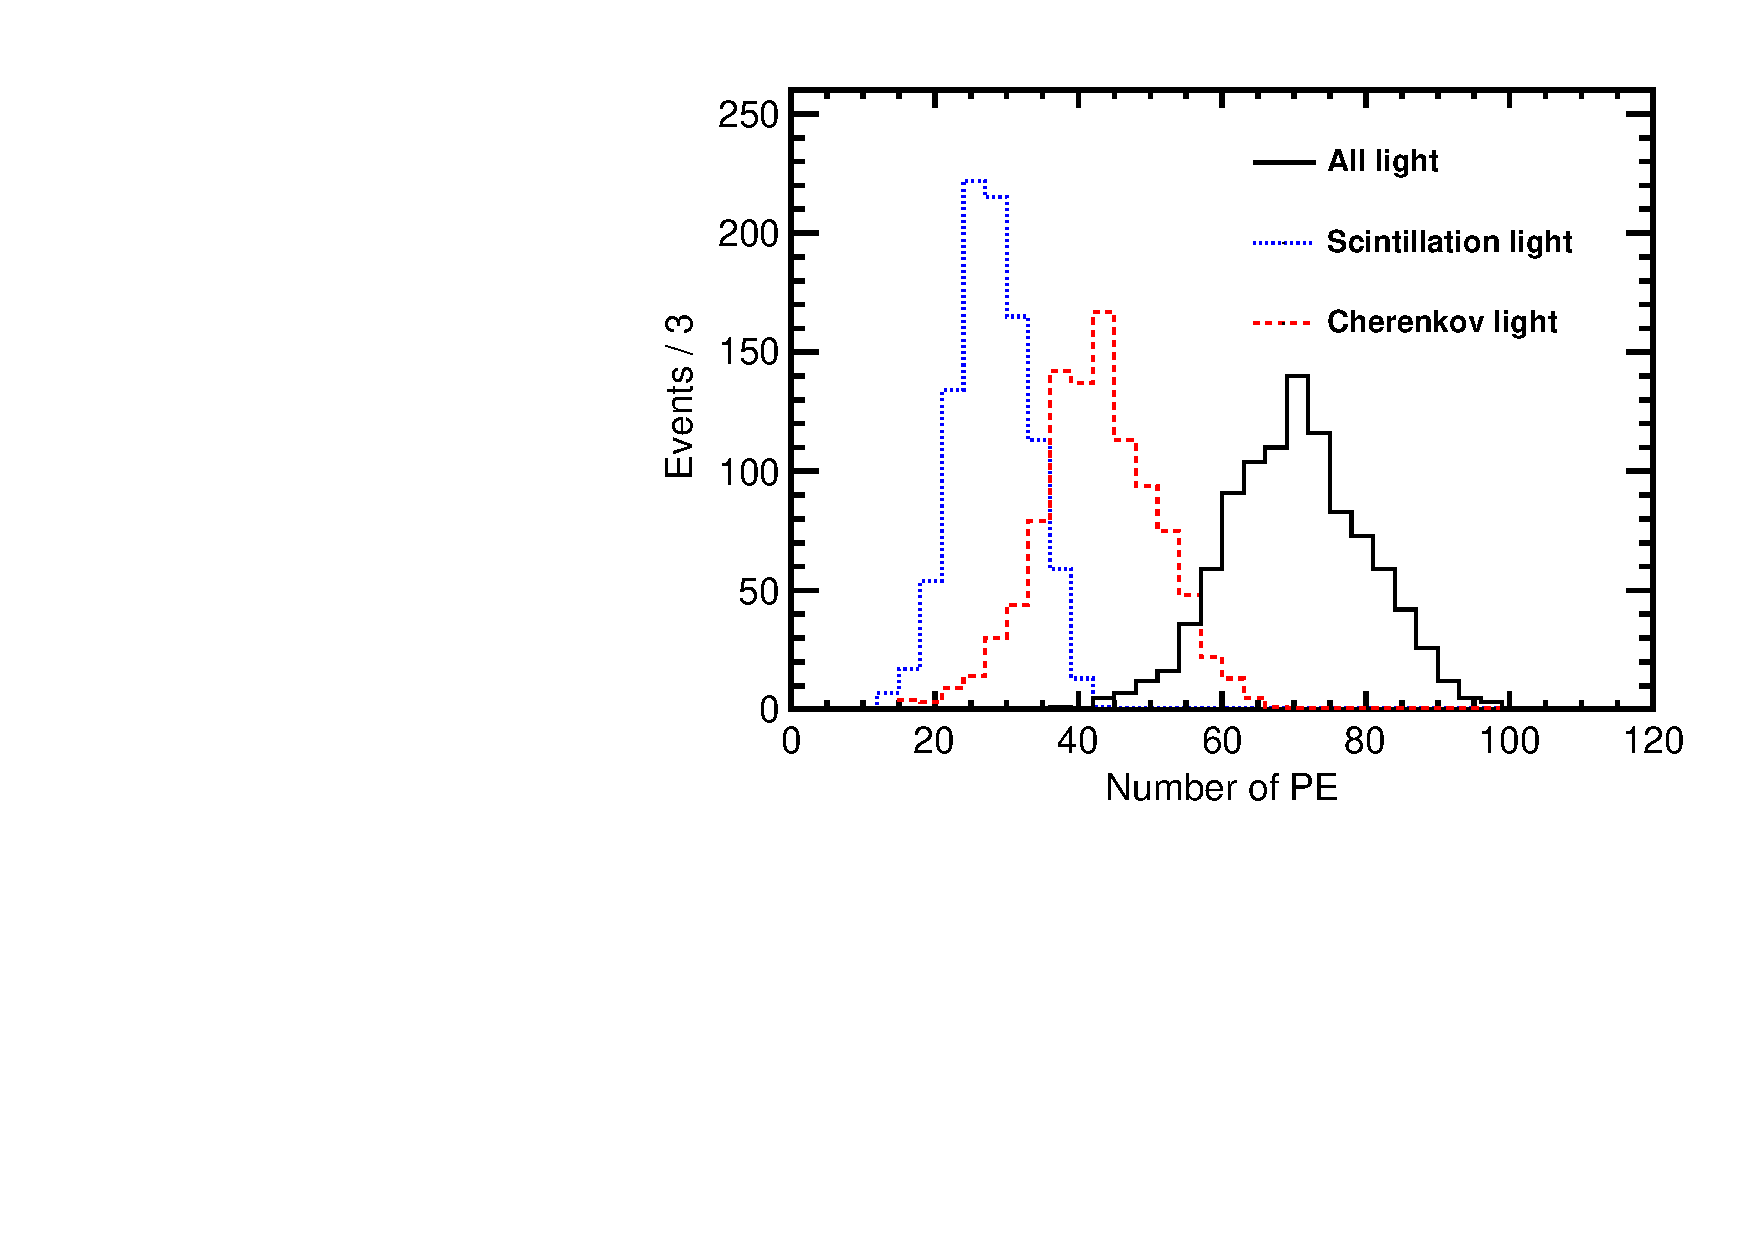
\includegraphics[width=0.45\textwidth]{hMomNPhot_1el_2p529MeV.pdf}
  \caption{\emph{Left:} A `zoomed-in' view of the photo-electron (PE)
   arrival times of signal and background events produced at the
   center of the detector.  The distribution in time for Cherenkov
   PEs from \Te 0\nbb is shown in solid black; Cherenkov PEs from
   \B~ solar neutrino background are shown in dashed red. PEs from
   scintillation are shown as the blue solid line. The line at 33.5~ns
   indicates the cut for the early PE sample selection.  \emph{Right:}
   Composition of the early PE sample: the number of Cherenkov PEs
   (\emph{dashed red line}), scintillation PEs (\emph{dotted blue
   line}), and total (\emph{solid black line}) PEs per event.}

\label{fig:ArrivalTimeDist_B8}
\end{figure*}


On average each \B~ neutrino event produces 69.9$\pm$0.3 PEs in the
early PE sample, with an RMS distribution width of 9.7 PEs due to
event-by-event fluctuations.  On average the early PE sample consist
of 27.6$\pm$0.2 scintillation and 42.3$\pm$0.3 Cherenkov PEs, with
event-by-event fluctuations contributing an RMS width of 5.2 and 8.2
PEs, respectively.  The total energy deposited in the detector in \B~
solar neutrino and 0\nbb-decay events is the same. This leads to
nearly the same amount of scintillation light produced in the
detector.

The number of Cherenkov photons is $\sim$10\% higher for \B~neutrino
events compared to 0\nbb-decay events. This is because Cherenkov light
in \B~ neutrino interactions is being produced by a single electron,
while the same kinetic energy is split between two electrons in
0\nbb-decay events~\footnote{We do not use the small difference in the
total number of PEs in the early PE sample due to the Cherenkov PE
contribution to separate 0\nbb-decay signal from \B~background.
However, it may provide an extra handle on signal-background
separation in a multivariate analysis when combined with directional
and topographical information.}.

